\subsection{Solutions proposées}

\paragraph{}Ces demandes font une bonne base pour un début de réflexion. Nous avons travaillé en étroite collaboration avec les chercheurs afin de leur proposer les solutions les plus
pertinentes. En parallèle, nous avons aussi servi de sujet à leurs tâches d'entrainement. Cela nous a permis de bien comprendre par quels procédés l'entrainement de l'attention était
possible et comment nous pouvions l'adapter à un jeu.

\subsubsection{Les mini jeux}

\paragraph{}Notre réflexion s'est d'abord porté sur le style de jeu. Nous avions besoin de confronter le joueur a divers contextes et gameplay pour pouvoir généraliser
son apprentissage. Nous en sommes venu à la conclusion que le mieux était de faire un ensemble de mini jeux. Pour leur réalisation, nous avions deux possibilités : garder le principe
de la tâche tout en la modifiant pour la gamifier, ou bien juste habiller la tâche.

Comme nous avons fait le choix de réaliser plusieurs mini jeux, nous avons préféré partir sur l'idée de garder le principe de la tâche en la modifiant. En effet, les mini jeux doivent
différer pour améliorer l'apprentissage.

\paragraph{}Des idées de mini jeux nous sont venus à l'esprit assez rapidement :
\begin{itemize}
\item Boxeur : identifiant les coups de l'adversaire pour choisir les bonnes actions (éviter, frapper ...)
\item Sonore : reconnaitre un son parmi une foule de sons distincts
\item Carrousel : un carrousel d'images défile avec des formes et couleurs semblables. Il faut reconnaitre une image en particulier.
\item Flèche : reprise de la tâche de CPT et se servir de l'orientation pour atteindre une cible
\item Runner : runner classique avec des objets du décor à éviter, en rajoutant des objets à récupérer comme Mario kart qui défilent dans une boite
\item Asterix : reconnaitre des romains (cible) qui apparaissent et disparaissent et les taper rapidement, il faut faire attention à ne pas taper les gaulois (distracteurs)
\item Tubes : des objets tombent à l'intérieur d'un tube ouvert, il faut retirer certains objets
\end{itemize}

\paragraph{}Après une réflexion plus poussée, nous avons approfondi certaines idées, oublié les autres, et trouvé de nouvelles. Nous avons également choisi un thème pour notre jeu qui
donne une ambiance intéressante : la \gls{SF}. C'est un thème qui parle beaucoup aux jeunes et qui permet de justifier facilement les environnements et les différents mini jeux.


\begin{wrapfigure}[11]{l}{6cm}
    \vspace{-25pt}
    \begin{center}
    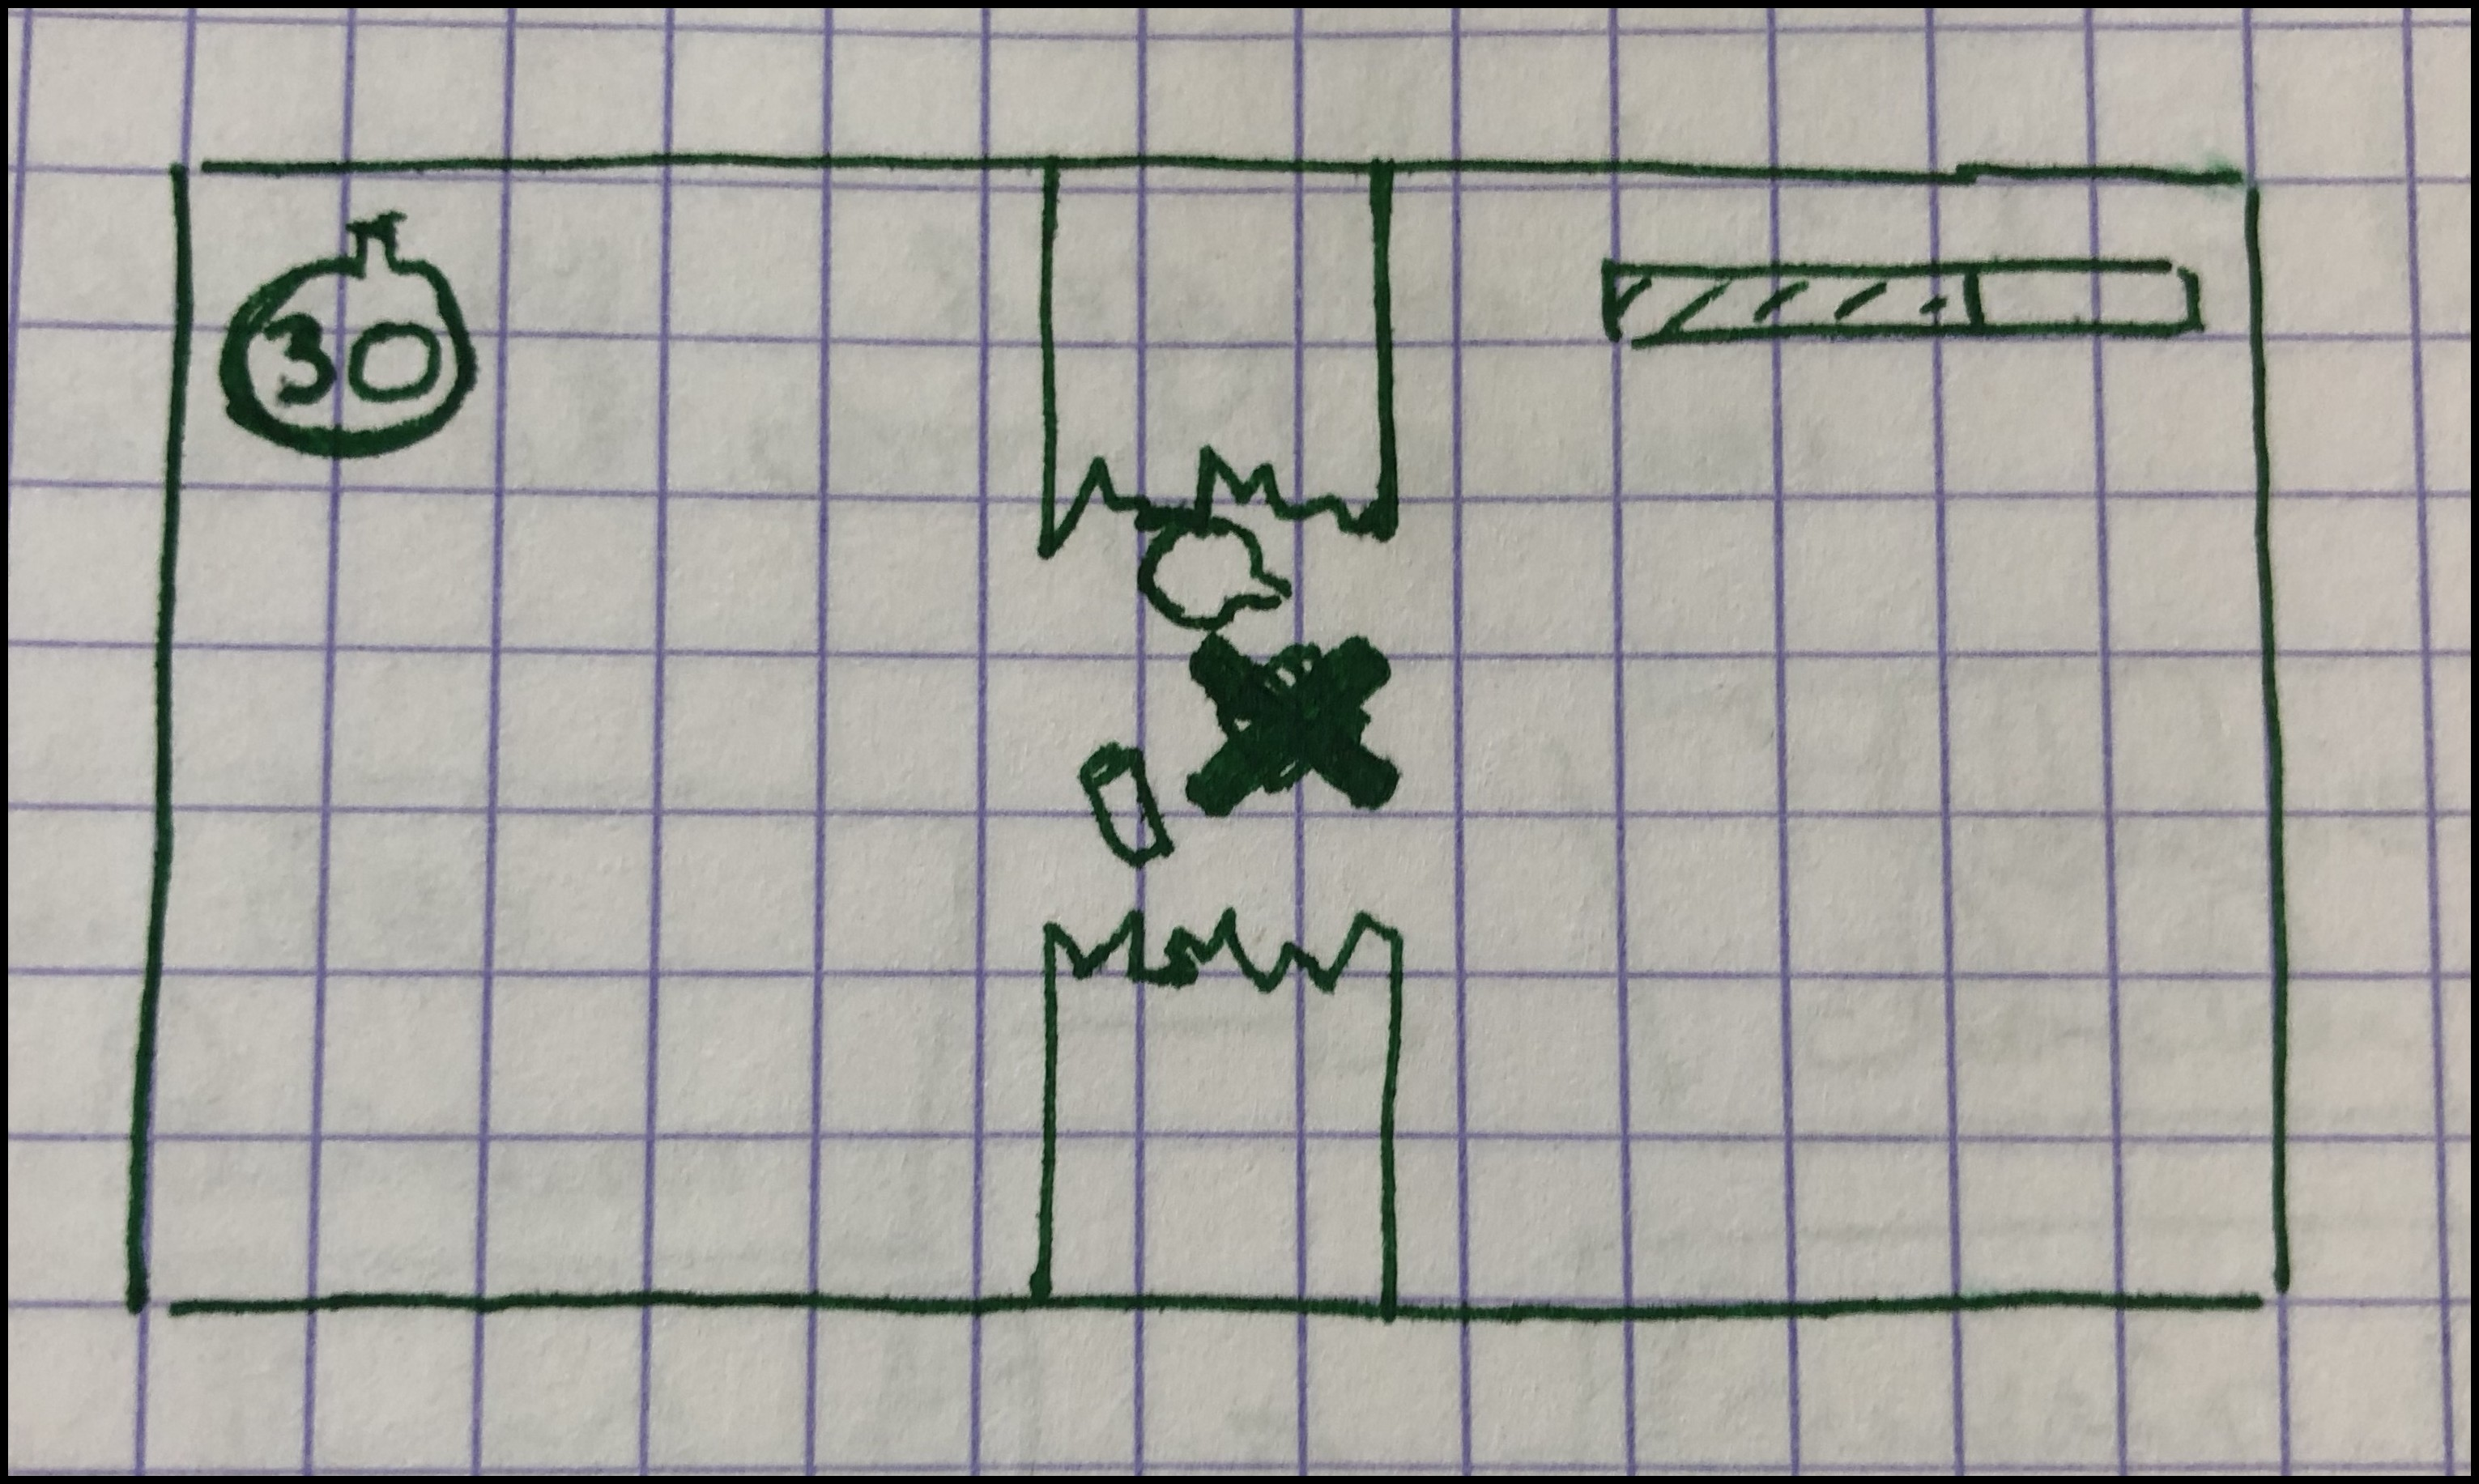
\includegraphics[width=6cm]{miniPipeConcept.jpg}
    \end{center}
    \captionsetup{labelformat=simpleNumber}
    \caption{Concept mini pipe}
\label{MiniPipeConcept}
\end{wrapfigure}

\paragraph{Mini pipe}Le mini jeu du tube était relativement simple. L'idée est que le joueur incarne un mécanicien qui est confronté à une panne dans la machine de tri des matériaux d'un
entrepôt. Il doit alors enlever les matériaux dangereux à la main le temps que les technicien réparent la panne. Le joueur doit donc reconnaitre très rapidement les matériaux qui
défilent pour retirer le bon. Cette mécanique assez proche de la tâche de CPT nous plaisant, nous avons décidé de la pousser plus loin pour en faire notre premier prototype. Mais nous
en parlerons plus en détail dans la partie \ref{prototypage}.

\begin{wrapfigure}[11]{l}{6cm}
    \vspace{-25pt}
    \begin{center}
    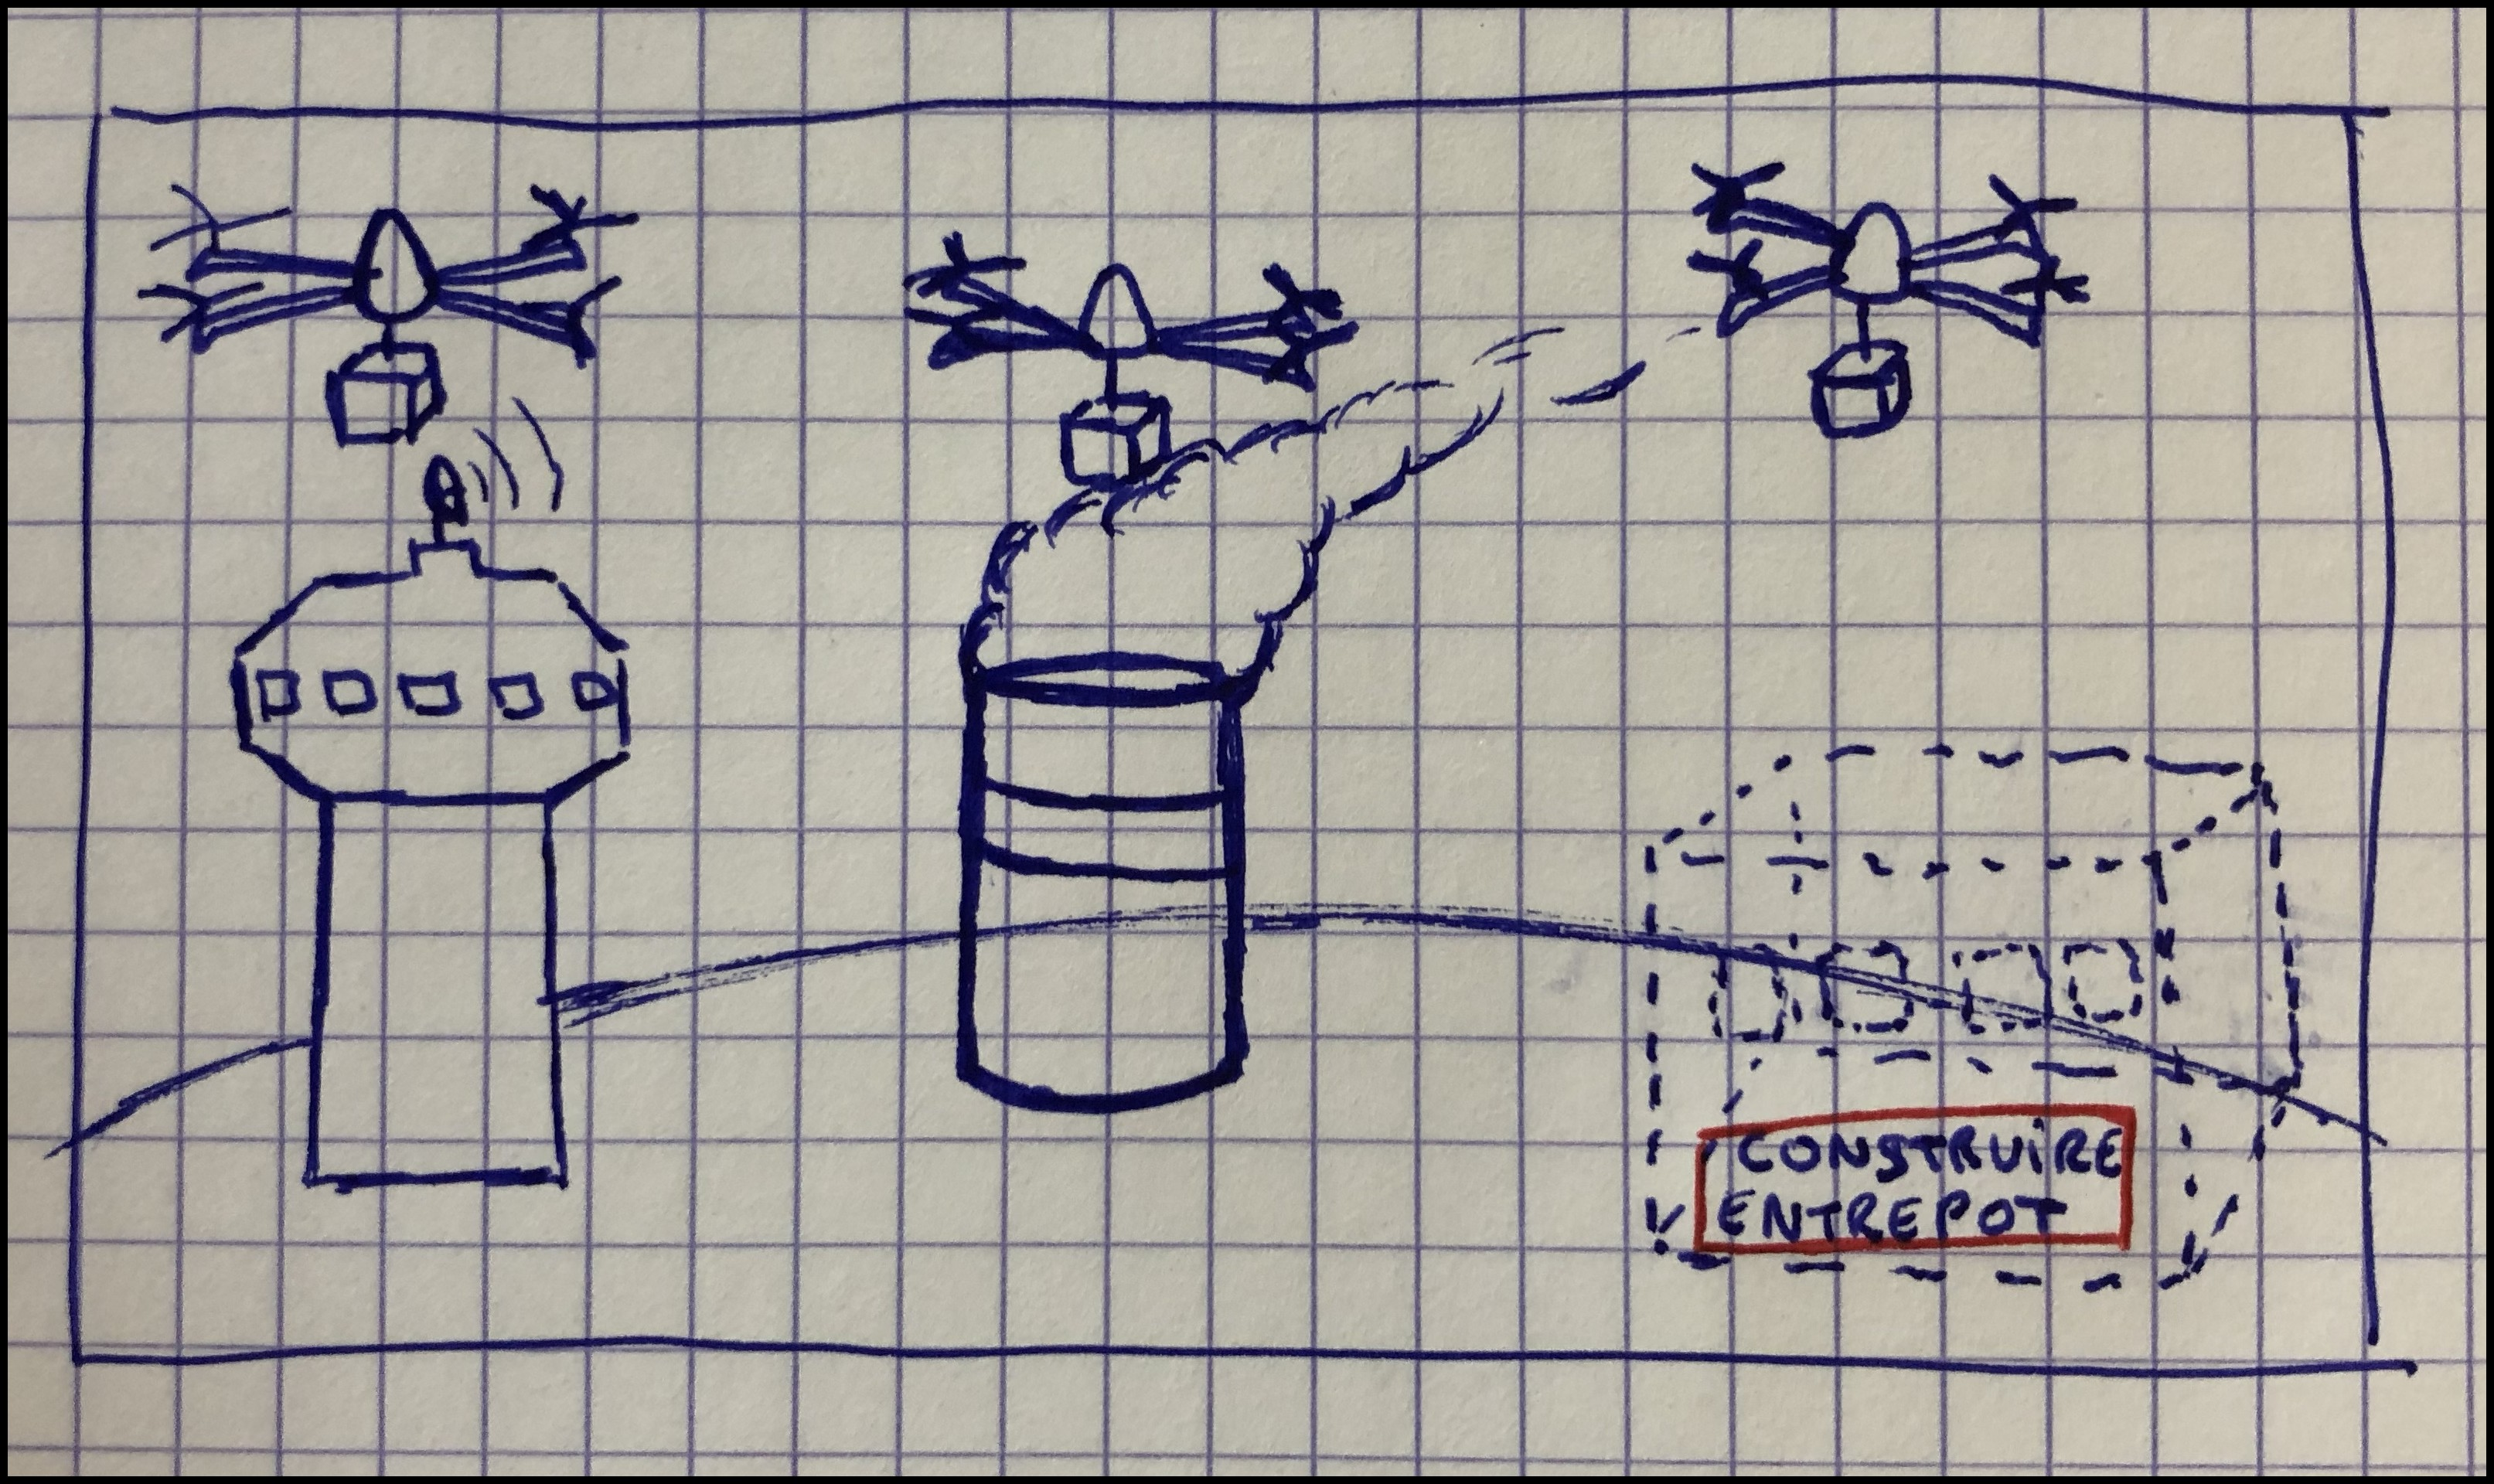
\includegraphics[width=6cm]{drones.jpg}
    \end{center}
    \captionsetup{labelformat=simpleNumber}
    \caption{Mini jeu drones}
\label{Drones}
\end{wrapfigure}

\paragraph{Les drones (anciennement Asterix)} Pour coller au thème de la \gls{SF}, les romains sont devenus des drones. Dans un premier temps, nous avons pensé à envoyer des matériaux
au bons drones. Puis, pour complexifier le mini jeu, nous avons rajouté des éléments de gameplay. Tel un architecte, le joueur doit au contraire récupérer les matériaux dont
il a besoin aux drones correspondant. Le joueur doit avec les matériaux construire les bâtiments d'une base scientifique. Chaque bâtiment nécessite certains matériaux et rapporte un
nombre de points de score défini. Il pourra éventuellement améliorer les bâtiments. Ceux-ci joueront également un rôle dans l'apparition des matériaux. Il devra donc porter son
attention sur plusieurs choses à la fois : les drones qui passent et la construction des bâtiments.

\newpage

\begin{wrapfigure}[17]{l}{6cm}
    \vspace{-10pt}
    \begin{center}
    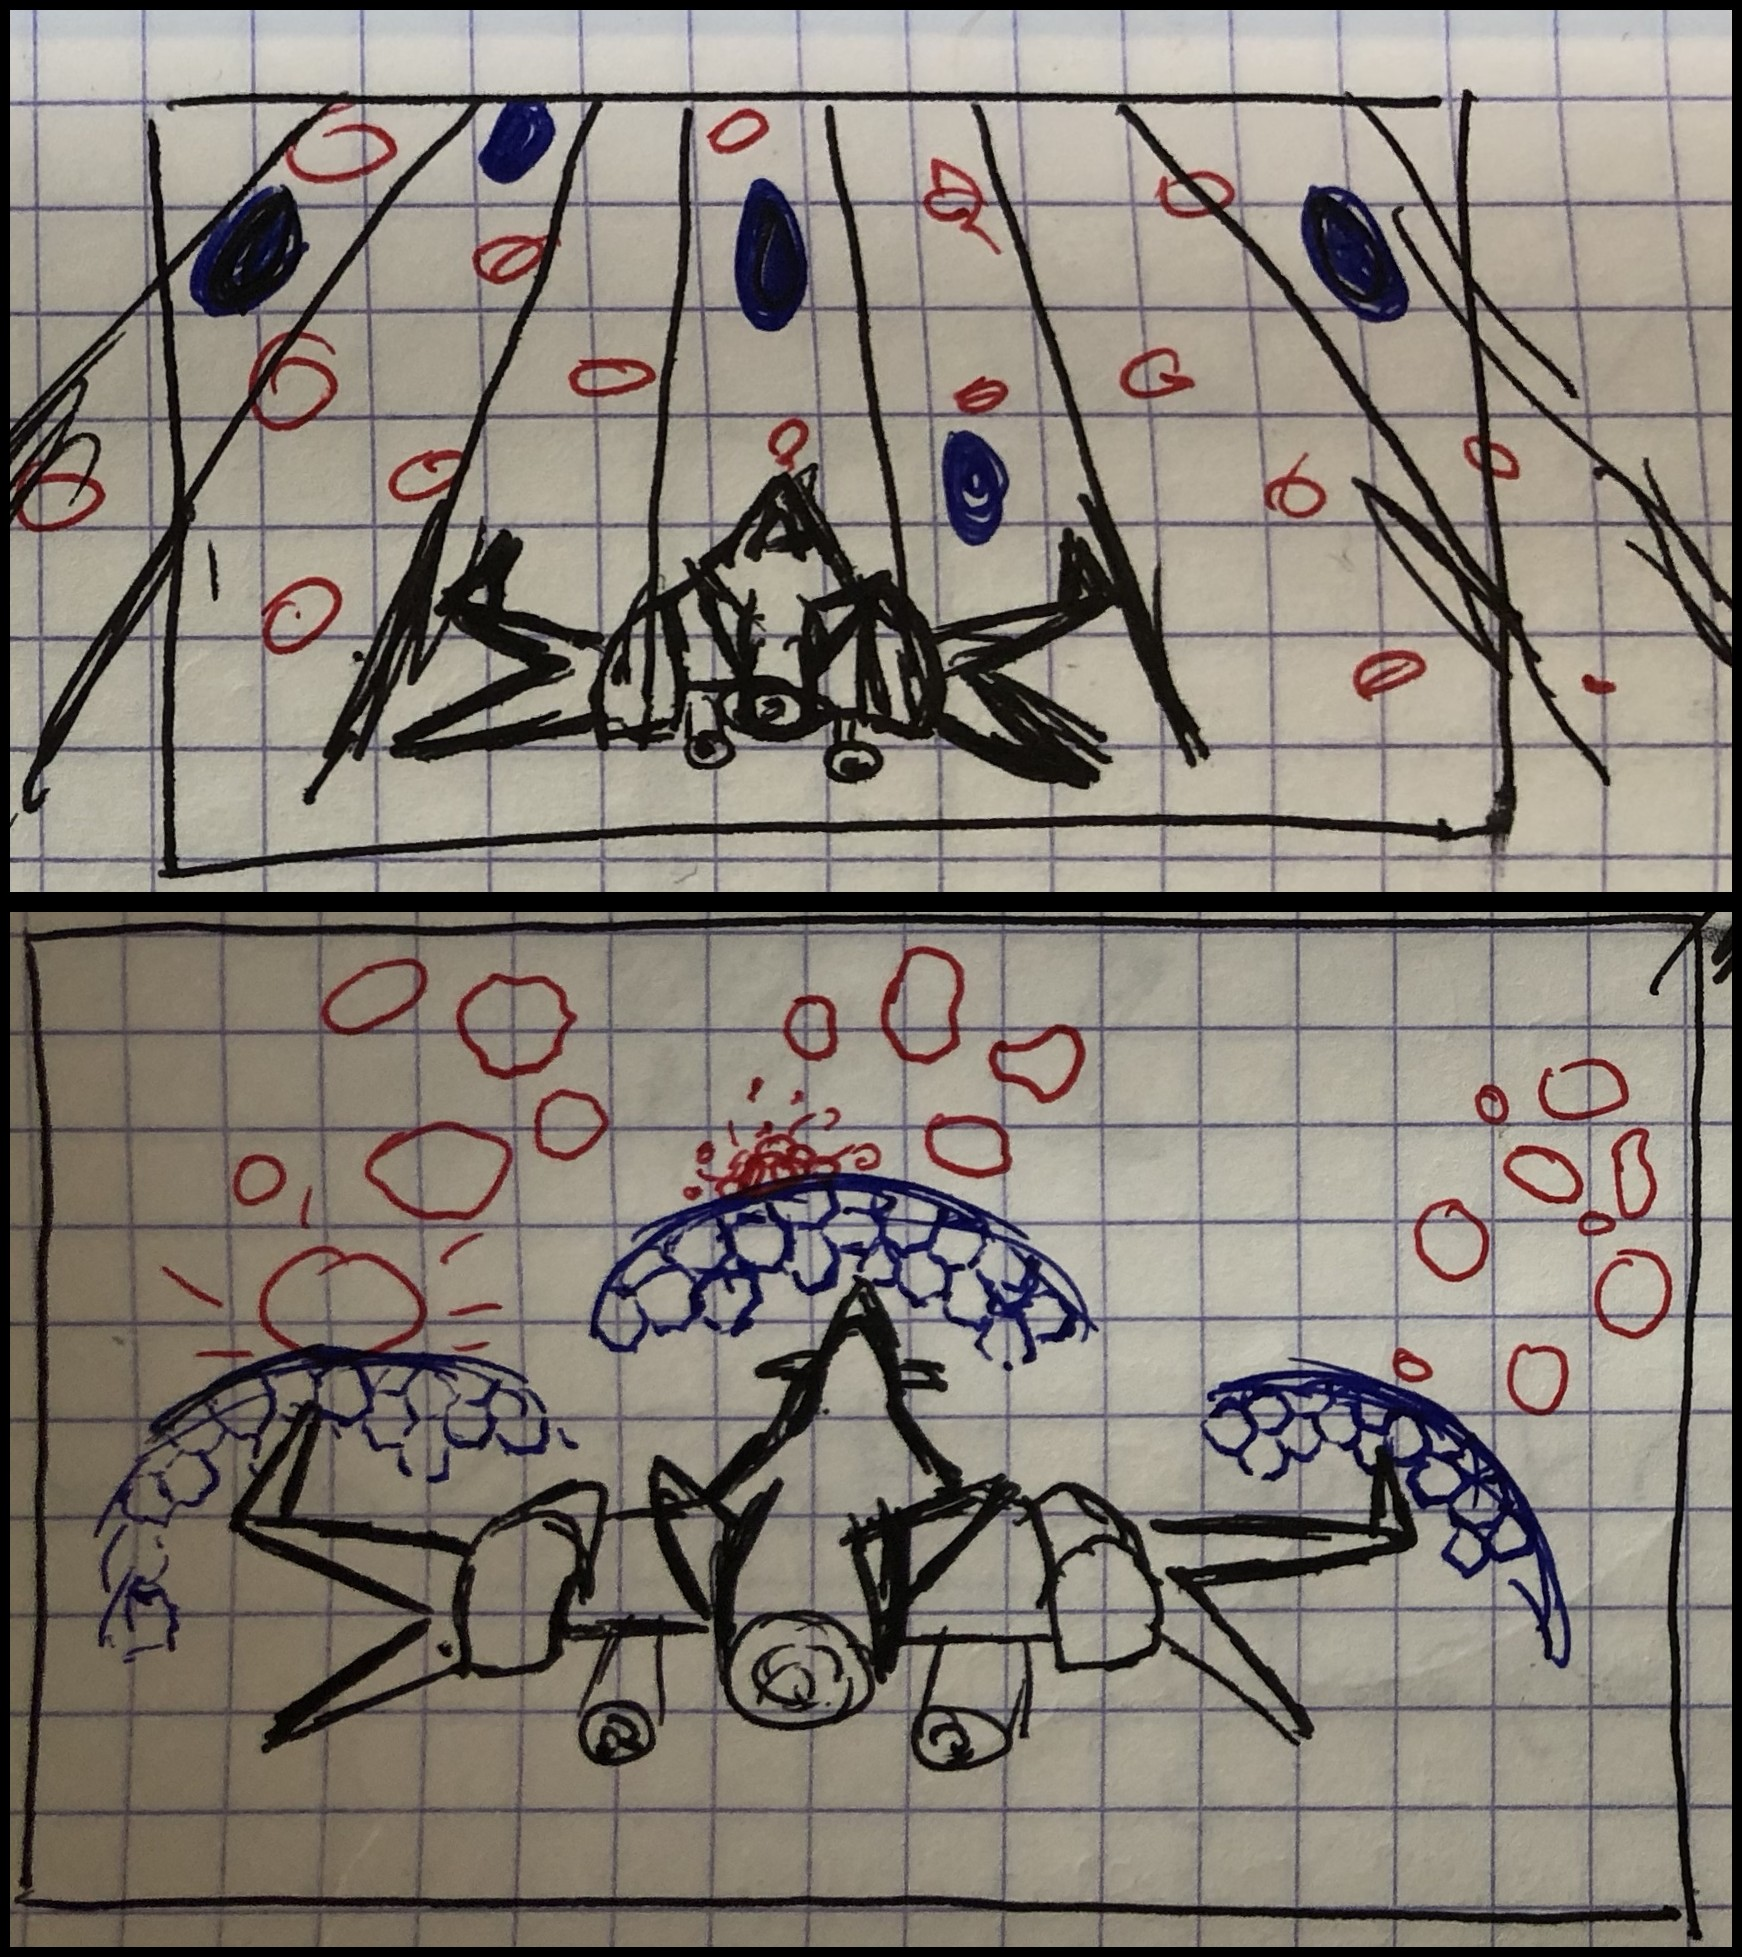
\includegraphics[width=6cm]{spaceship.jpg}
    \end{center}
    \captionsetup{labelformat=simpleNumber}
    \caption{Mini jeu Spaceship}
\label{Spaceship}
\end{wrapfigure}

\paragraph{Spaceship (anciennement Runner)}Le joueur contrôle un vaisseau spatial qui parcourt l'univers. Sur sa route, il croise des météores à éviter qui causent des dommages au
vaisseau, et des naufragés dans des capsules de secours à secourir. Il peut se déplacer à droite ou à gauche pour éviter les météores et dispose d'une recharge de bouclier qu'il peut
placer soit sur l'avant du vaisseau, soit à droite, soit à gauche. Ce bouclier est à utiliser avec parcimonie car il empêche la récupération des naufragés. On peut imaginer une
compétence spéciale qui se recharge au cours du temps, ou au fur et à mesure que le joueur récupère des naufragés. Elle pourrait permettre de détruire tous les météores affichés en
envoyant des missiles téléguidés.


\newpage
\subsubsection{Contexte}

\paragraph{Les mondes}Une des premières discussions concernant le jeu a mis en avant l'importance de faire évoluer le jeu de manière a entrainer petit à petit le joueur a chaque aspect
de l'attention. En effet, le joueur doit d'abord pouvoir se concentrer dans la durée sur un point centrale fixe. Quand il y arrive, on peut essayer de faire bouger son attention dans
l'espace ... Nous en avons conclu qu'il fallait un "monde" par aspect de l'attention à entrainer. Quatre aspects ont été retenus comme mondes :
\begin{itemize}
\item l'attention soutenue
\item l'attention \textcolor{red}{A COMPLETER}
\item l'attention divisive
\item l'attention exécutive
\end{itemize}

\paragraph{}Décrire les niveaux des mondes

\paragraph{Les scénarios} rattachement aux matières -> 1 scénario par matière. Un même monde dans 2 scénarios : 2 mini jeu en apparence différent mais avec des mécaniques assez
semblables

\subsubsection{Le multijoueur}



Protocole : pas intéressant -> jeu intéressant, voir addictif

1 monde = 1 aspect de l'attention -> plusieurs mini jeux pour chaque aspect
progression adaptée à chaque joueur
jeu à faire en cours -> relier les mini jeux à des matières pour intéresser les professeurs

aspect multi : coopération en petits groupes et compétition entre les groupes (inclure le professeur dans le gameplay)